\begin{frame}{Metodologia -- Dados Experimentais}
\begin{itemize}
    \item \alert{Base da dados}: Imagens do exame microscópico de lâminas de sangue no Hospital Universitário  Chittagong, Bangladesh.
    \ \ \newline
    \item $1830$ imagens de $150$ pacientes
    \item Arquivo de rótulo por imagem
    \item Células brancas e protozoários ($84509$)
    \item Delimitação dos objetos em formato circular
\end{itemize}
\end{frame}

\begin{frame}{Metodologia -- Dados Experimentais}
\begin{figure}[H]
    \centering
	\hfill \subfloat[Imagem original]{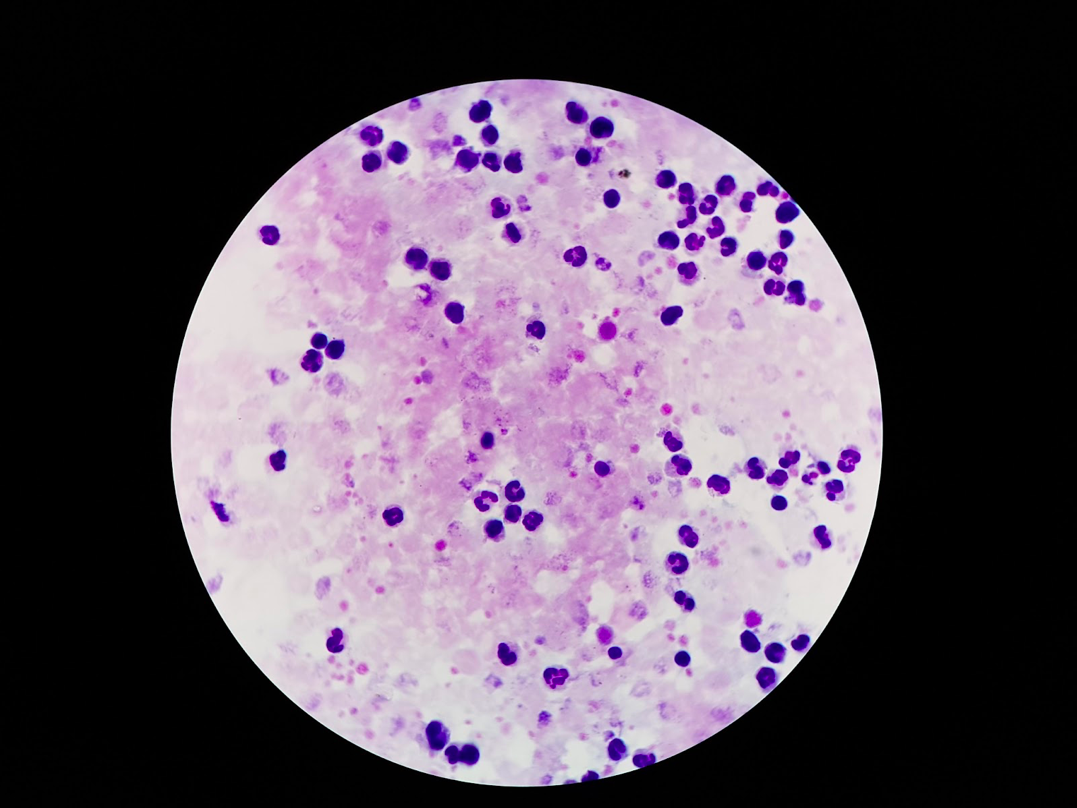
\includegraphics[width=0.4\linewidth]{./img/sample.png}} \hfill \subfloat[Imagem rotulada]{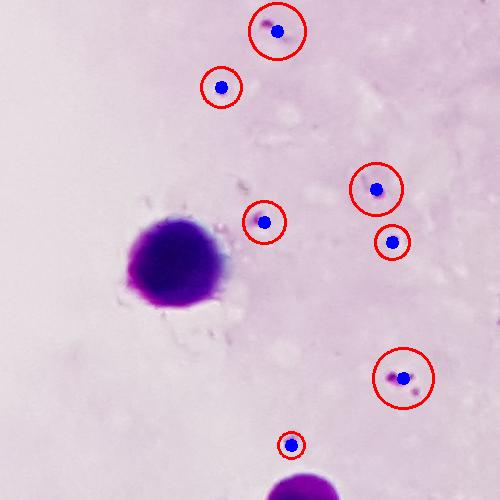
\includegraphics[width=0.35\linewidth]{./img/blood-circles.jpg}}\\
	\caption{Exemplos de imagens originais e recortadas contendo os rótulos da classe protozoário.} \label{img:dataset-samples}
\end{figure}
\end{frame}

\begin{frame}{Metodologia -- Distribuição das caixas delimitadoras}
\begin{figure}[H]
    \centering
    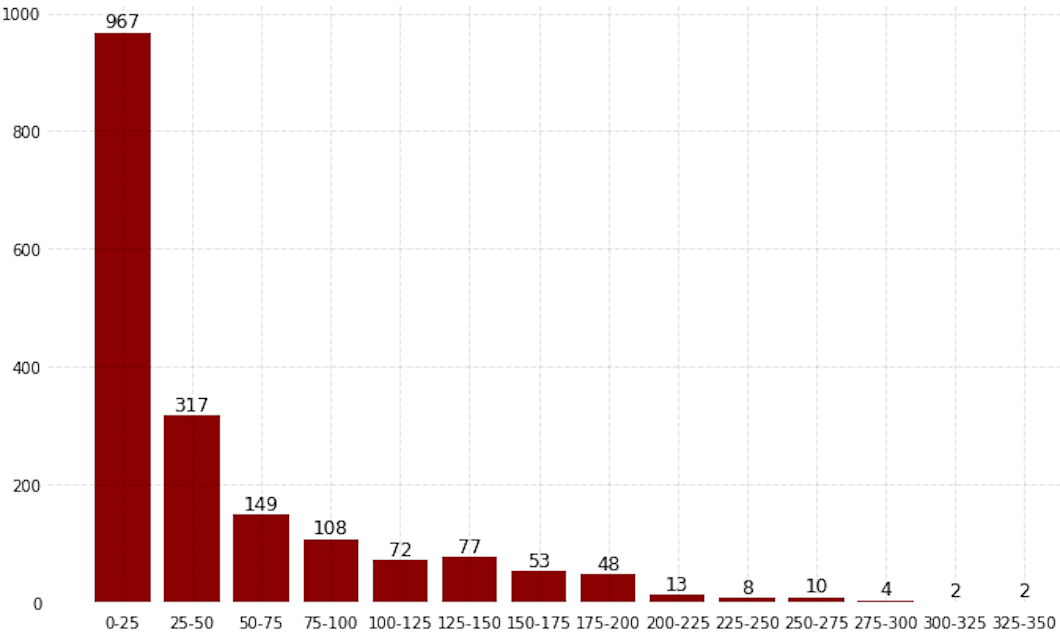
\includegraphics[width=0.65\linewidth]{./img/histogram.png}
    \caption{Histograma do número de caixas delimitadoras por imagem.}
    \label{fig:histogram}
\end{figure}
\end{frame}

\begin{frame}{Metodologia -- Regiões das caixas delimitadoras}
\begin{figure}[H]
    \centering
    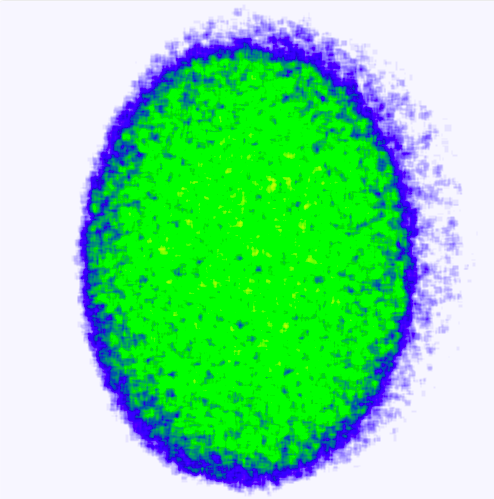
\includegraphics[width=0.5\textwidth,height=0.375\textwidth]{./img/heat-map.png}
    \caption{Mapa de calor da distribuição das caixas delimitadoras pela área da imagem.}
    \label{fig:heat-map}
\end{figure}
\end{frame}

\begin{frame}{Metodologia --  Validação e Avaliação}
\begin{itemize}
\item Validação Cruzada do tipo \alert{\emph{holdout}}
\begin{itemize}
    \item Treinamento: $70\%$
    \item Validação: $10\%$
    \item Teste: $20\%$
\end{itemize}
\ \ \newline
\item Regularização com o uso de \alert{\emph{early stopping}: $100$ épocas} na YOLOv5
\item \alert{Métricas}: Precisão, Revocação, $F_1$-\emph{Score} e mAP@0.5
\end{itemize}
\end{frame}

\begin{frame}{Metodologia -- Parâmetros e Hiperparâmetros}
\begin{itemize}
    \item \alert{YOLOv5} \emph{Nano}: $\num{1,7}$ milhões
    \item \alert{YOLOv5} \emph{Small}: $\num{7}$ milhões 
    \item \alert{YOLOv5} \emph{Medium}: ${20,8}$ milhões
    \ \ \newline
    \item \alert{YOLOv7} \emph{Tiny}: $\num{6}$ milhões
    \item \alert{YOLOv7} \emph{Standard}: $\num{36,4}$ milhões
    \item \alert{YOLOv7} \emph{Large}: $\num{70,7}$ milhões
    \ \ \newline
    \item Número de épocas: $300$ e $500$ épocas
    \item Taxa de aprendizado: $10^{-2}$
    \item Tamanho do \emph{batch}: $16$, $8$ e $4$
\end{itemize}
\end{frame}


